\documentclass[12pt]{article}
\usepackage{amsmath}
\usepackage{amssymb}
\usepackage{graphicx}
\usepackage{geometry}\usepackage{hyperref} % Enables hyperlinks in the document

\hypersetup{
    colorlinks=true,       % Enable colored links
    linkcolor=black,        % Color for internal links (e.g., TOC)
    urlcolor=cyan,         % Color for URLs
    citecolor=red          % Color for citations
}
\geometry{margin=1in}

\title{Padeye and Spreader Bar Design Report}
\author{Quang Anh To}
\date{\today}

\begin{document}

\maketitle

\tableofcontents

\pagebreak
\section{Introduction}
This report summarizes the padeye design checks, including geometric, bearing, and shear stress verifications, using the provided dimensions and material properties. All calculations are shown in plain text and equations for clarity.

\subsection*{Padeye design details}
\begin{center}
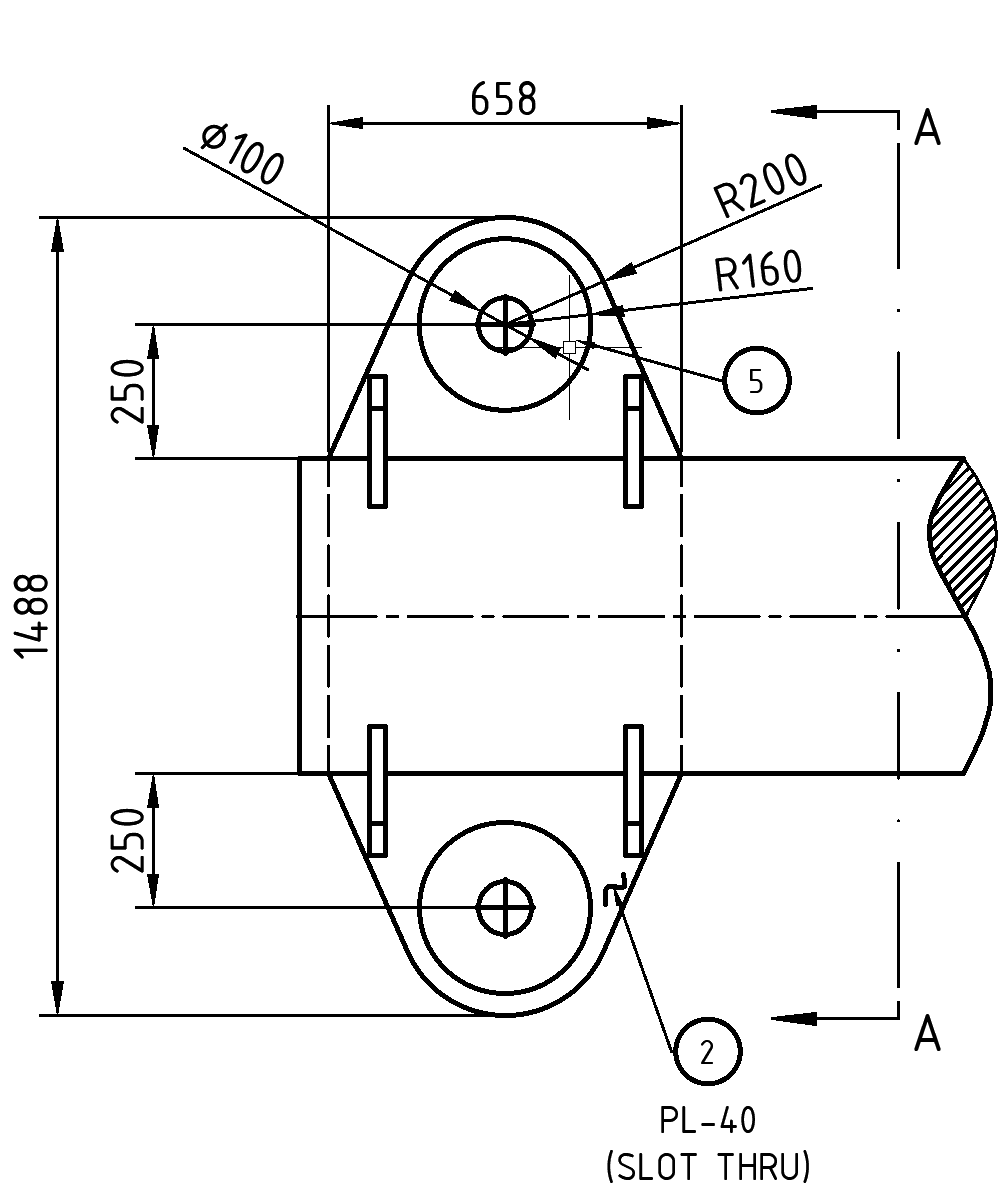
\includegraphics[width=0.6\textwidth]{image-1.png}
\end{center}

\section{Input Data}
\begin{itemize}
  \item Shackle Pin Diameter: $D = 95\ \mathrm{mm}$ (GreenPin P-6036 WLL: 120 MT)
  \item Shackle Jaw Opening Width: $B = 147\ \mathrm{mm}$
  \item Shackle Inside Length: $H = 329\ \mathrm{mm}$
  \item Sling Diameter: $D_s = 80\ \mathrm{mm}$
  \item Yield Strength of Material: $F_y = 345\ \mathrm{MPa}$
  \item Young's Modulus: $E = 210,000\ \mathrm{MPa}$
  \item Poisson's Ratio: $\nu = 0.3$
  \item Padeye Hole Diameter: $d = 100\ \mathrm{mm}$
  \item Main Plate Thickness: $t = 40\ \mathrm{mm}$
  \item Cheek Plate Thickness: $t_c = 30\ \mathrm{mm}$
  \item Provided Main Plate Radius: $R_p = 200\ \mathrm{mm}$
  \item Provided Cheek Plate Radius: $R_c = 160\ \mathrm{mm}$
  \item Total Plate Thickness: $t_p = 100\ \mathrm{mm}$
  \item Padeye Length: $L = 658\ \mathrm{mm}$
  \item Number of Stiffeners: $n_{stiff} = 4$
  \item Distance Between Stiffener Centers: $H_s = 478\ \mathrm{mm}$
  \item Sling Load: $S_l = 86\ \mathrm{MT}$
  \item Acceleration due to Gravity: $g = 9.81\ \mathrm{m/s^2}$
  \item Calculated Sling Load: $SSL = S_l \times g \times 1,000 = 86 \times 9.81 \times 1,000 = 843,660\ \mathrm{N}$
\end{itemize}

\section{Geometric Checks}
\subsection{Clearance Between Hole and Pin}
Pin Diameter: $d = 95\ \mathrm{mm}$\\
Hole Diameter: $D = 100\ \mathrm{mm}$\\
Clearance: $C_1 = D - d = 100 - 95 = 5\ \mathrm{mm}$

\subsection{Clearance Between Shackle Jaw and Plate}
Shackle Jaw Opening: $B = 147\ \mathrm{mm}$\\
Total Plate Thickness: $t_p = 100\ \mathrm{mm}$\\
Clearance: $C_2 = \frac{B - t_p}{2} = \frac{147 - 100}{2} = 23.5\ \mathrm{mm}$

\subsection{Sling Clearance}
Sling Clearance: $SC = H - (D_s + R_p - 0.5 \cdot d) = 329 - (80 + 200 - 0.5 \times 100) = 329 - 280 = 49\ \mathrm{mm}$

\subsection{Minimum and Maximum Hole Sizes}
Minimum Hole: $\text{Minimum Hole} = \max(D + 3.18,\ 1.05 \cdot D) = \max(95 + 3.18,\ 1.05 \times 95) = \max(98.18,\ 99.75) = 99.75\ \mathrm{mm}$\\
Maximum Hole: $\text{Maximum Hole} = D + 9.53 = 95 + 9.53 = 104.53\ \mathrm{mm}$

\subsection{Minimum and Maximum Clearances}
Minimum Clearance: $\text{Minimum Clearance} = 0.05 \times t_p = 0.05 \times 100 = 5\ \mathrm{mm}$\\
Maximum Clearance: $\text{Maximum Clearance} = \max(0.1 \times t_p,\ 20) = \max(10,\ 20) = 20\ \mathrm{mm}$

\section{Bearing Stress Check}
Applied Load: $F = SSL = 843,660\ \mathrm{N}$\\
Padeye Hole Diameter: $d = 100\ \mathrm{mm}$\\
Main Plate Thickness: $t = 40\ \mathrm{mm}$\\
Bearing Stress:
\[
\sigma_b = \frac{F}{d \cdot t} = \frac{843,660}{100 \times 40} = 210.92\ \mathrm{MPa}
\]
Permissible Bearing Stress:
\[
\sigma_{b,\text{perm}} = 0.9 \times F_y = 0.9 \times 345 = 310.5\ \mathrm{MPa}
\]
Check: $210.92\ \mathrm{MPa} < 310.5\ \mathrm{MPa} \implies \text{PASS}$

\section{Case 1 Check shear failure from pin hole through main/cheek plate}
\begin{center}
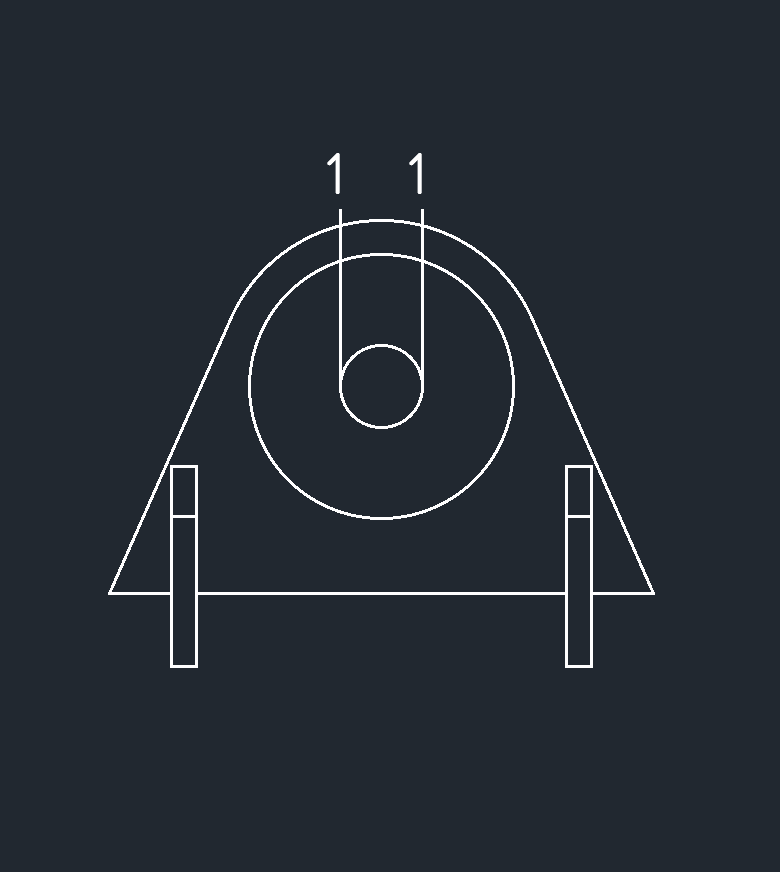
\includegraphics[width=0.5\textwidth]{image-2.png}
\end{center}
Applied Load: $F = SSL = 843,660\ \mathrm{N}$\\
Main Plate Radius: $R_p = 200\ \mathrm{mm}$\\
Cheek Plate Radius: $R_c = 160\ \mathrm{mm}$\\
Shackle Hole Diameter: $d = 100\ \mathrm{mm}$\\
Main Plate Thickness: $t = 40\ \mathrm{mm}$\\
Cheek Plate Thickness: $t_c = 30\ \mathrm{mm}$\\
Resisting Area:
\[
A_{p1} = (R_p - \frac{d}{2}) \times 2t + (R_c - \frac{d}{2}) \times 4t_c = 25,200\ \mathrm{mm}^2
\]
Shear Stress:
\[
\sigma_s = \frac{F}{A_{p1}} = \frac{843,660}{25,200} = 33.49\ \mathrm{MPa}
\]
Permissible Shear Stress:
\[
\sigma_{s,\text{perm}} = 0.4 \times F_y = 0.4 \times 345 = 138\ \mathrm{MPa}
\]
Check: $33.49\ \mathrm{MPa} < 138\ \mathrm{MPa} \implies \text{PASS}$

\section{Case 2: Shear Stress Failure in Main Plate}
\begin{center}
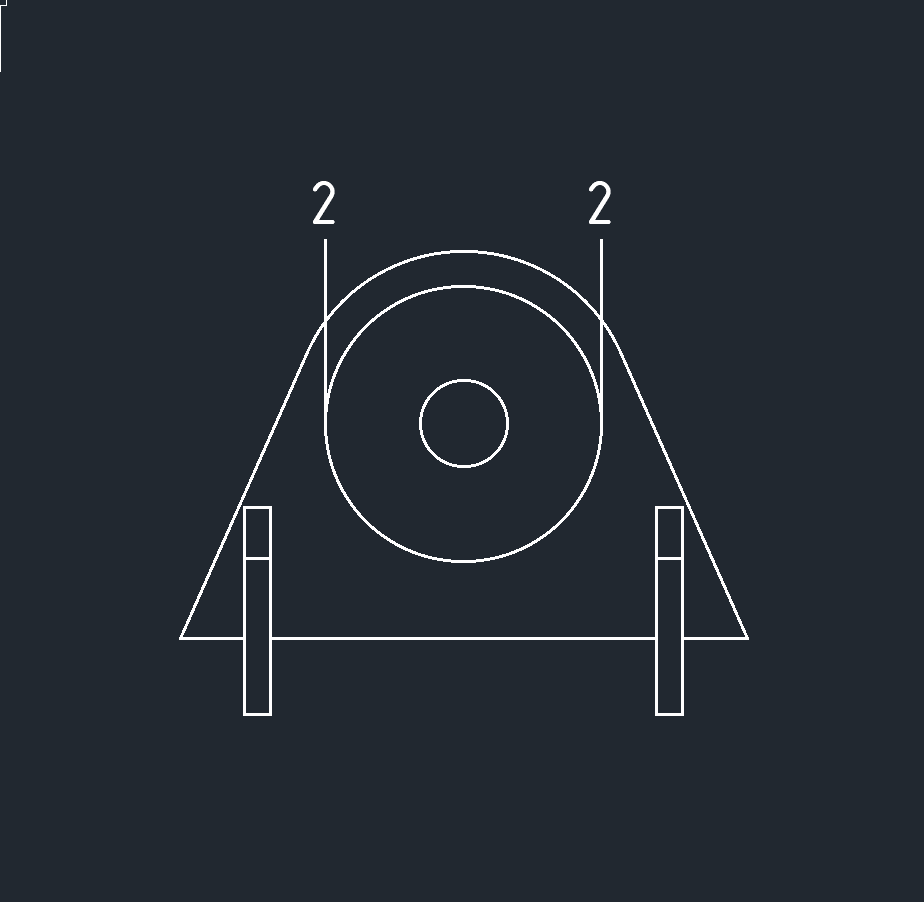
\includegraphics[width=0.6\textwidth]{Case2.png}
\end{center}

The allowable shear stress is:
\(
0.4 \cdot F_{y} = 138\ \mathrm{MPa}
\)

The resisting area of the plate is calculated as:
\[
A_{p2} = (R_p - R_c) \cdot 2t + \pi R_c t
\]
Where:
\begin{itemize}
  \item $R_p$ = 200 mm (Provided main plate radius)
  \item $R_c$ = 160 mm (Provided cheek plate radius)
  \item $t$ = 40 mm (Main plate thickness)
\end{itemize}

Substituting the values:
\[
A_{p2} = (200 - 160) \times 2 \times 40 + \pi \times 160 \times 40 = 3,200 + 20,106 = 23,306\ \mathrm{mm}^2
\]

The shear stress is:
\[
\tau_{v2} = \frac{F}{A_{p2}} = \frac{843,660}{23,306} = 36.22\ \mathrm{MPa}
\]
Where:
\begin{itemize}
  \item $F$ = 843,660 N (Load on the padeye)
  \item $A_{p2}$ = 23,306 mm$^2$ (Resisting area of the plate)
\end{itemize}

The check is:
\(
36.22\ \mathrm{MPa} < 138\ \mathrm{MPa} \implies \text{OK}
\)

Therefore, the main plate is safe against shear stress failure in this case.

\section{Summary Table}
\begin{center}
\begin{tabular}{|l|l|l|l|}
\hline
Check & Calculated Value & Permissible Value & Result \\
\hline
Bearing Stress ($\sigma_b$) & 210.92 MPa & 310.5 MPa & PASS \\
Shear Stress ($\sigma_s$) & 33.49 MPa & 138 MPa & PASS \\
Hole Size & 100 mm & 99.75 -- 104.53 mm & PASS \\
Clearance ($C_2$) & 23.5 mm & 5 -- 20 mm & FAIL \\
\hline
\end{tabular}
\end{center}

\section{Conclusion for padeye}
All checks except the shackle jaw clearance ($C_2$) are within permissible limits. The clearance between the shackle jaw and the plate exceeds the maximum allowed value and should be reviewed in the design.

\section{Spreader Bar Critical Stress}
The critical buckling load of the spreader bar is calculated as follows:

\subsection*{Step 1: Moment of Inertia}
The moment of inertia for a hollow circular section:
\[
I = \frac{\pi}{64} (D_o^4 - D_i^4)
\]
Where:
\begin{itemize}
  \item $D_o$ = Outer diameter = 588 mm
  \item $t$ = Thickness = 25 mm
  \item $D_i = D_o - 2t = 588 - 2 \times 25 = 538\ \mathrm{mm}$
\end{itemize}
So,
\[
I = \frac{\pi}{64} (588^4 - (588-2 \times 25)^4) = 1.75 \times 10^9\ \mathrm{mm}^4
\]

\subsection*{Step 2: Radius of Gyration}
\[
r = \sqrt{\frac{I}{A}}
\]
Where:
\[
A = \frac{\pi}{4} (D_o^2 - D_i^2)
\]

\subsection*{Step 3: Euler's Critical Buckling Load}
The critical buckling load for a pinned-pinned column:
\[
P_{cr} = \frac{\pi^2 E I}{(K L)^2}
\]
Where:
\begin{itemize}
  \item $E = 210,000\ \mathrm{MPa}$
  \item $K$ = 1 (effective length factor)
  \item $L = 6,288\ \mathrm{mm}$ (length of spreader bar)
\end{itemize}
Substituting the values:
\[
P_{cr} = \frac{\pi^2 \times 210,000 \times 1.75 \times 10^9}{(1 \times 6,288)^2} = 92,018,373.48\ \mathrm{N} = 9,383.26\ \text{Tons}
\]

\subsection*{Step 4: Comparison}
\begin{itemize}
  \item Calculated compressive force from rigging: $F_c = 37.43$ Tons
  \item Critical buckling load: $P_{cr,\text{tons}} = 9,383.26$ Tons
\end{itemize}
Since $F_c \ll P_{cr,\text{tons}}$, the spreader bar is safe against buckling under the given load.

\section{Allowable Axial Compressive Stress (ASME BTH-1 2008)}

The allowable axial compressive stress $F_a$ is calculated according to the AISC code, depending on the slenderness ratio $KL/r$:

\begin{itemize}
  \item If $KL/r \leq C_c$:
  \[
  F_a = \left[1 - \frac{(KL/r)^2}{2C_c^2}\right] \frac{F_y}{N_d} \left[1 + \frac{9(KL/r)}{40C_c} - \frac{3(KL/r)^3}{40C_c^4}\right] \ (eq. \ 3.3)
  \]
  \item If $KL/r > C_c$:
  \[
  F_a = \frac{\pi^2 E}{1.15 N_d (KL/r)^2} \ (eq. \ 3.5)
  \]
\end{itemize}

Where:
\begin{itemize}
  \item $F_y$ = 345 MPa (yield strength)
  \item $N_d$ = 4 (safety factor)
  \item $E$ = 210,000 MPa (Young's modulus)
  \item $K$ = 1 (effective length factor)
  \item $L$ = 6,288 mm (length)
  \item $r$ = 199.25 mm (radius of gyration)
  \item $C_c = \sqrt{\frac{2\pi^2 E}{F_y}} \ (eq. \ 3.4)$ 
\end{itemize}

Calculate $KL/r$ and $C_c$:
\[
KL/r = \frac{K \cdot L}{r} = \frac{1 \times 6,288}{199.25} = 31.56
\]
\[
C_c = \sqrt{\frac{2\pi^2 \times 210,000}{345}} = 109.61
\]
\\
Since $KL/r < C_c$, use the first formula:
\[
F_a = 88.03\ \mathrm{MPa} = 8.80\ \mathrm{MT/m^2}
\]

\textbf{Applied Compressive Stress Calculation:}

The applied compressive stress is calculated as:
\[
F_{\text{app}} = \frac{F}{A_s}
\]
Where:
\begin{itemize}
  \item $F = 367,062.90\ \mathrm{N}$ (compressive force)
  \item $A_s = 44,217.92\ \mathrm{mm}^2$ (cross-sectional area)
\end{itemize}
So,
\[
F_{\text{app}} = \frac{367,062.90}{44,217.92} = 8.30\ \mathrm{MPa}
\]

The allowable axial compressive stress is $F_a = 88.03$ MPa ($8.80$ MT/m$^2$).

The applied compressive stress from the rigging is:
\[
F_{\text{app}} = 8.30\ \mathrm{MPa} = 0.83\ \mathrm{MT/m^2}
\]

Since $F_{\text{app}} < F_a$, the applied compressive stress is within allowable limits and the spreader bar is safe under the applied compressive load according to ASME BTH-1 2008.

\end{document}
